\documentclass{article}
\usepackage{amsmath, amssymb, cite, algorithmic, url, braket}
\usepackage{graphicx}
\usepackage{pythonhighlight}
\usepackage[margin=1.5cm]{geometry}
\usepackage[title]{appendix}
\usepackage{subfigure}
\usepackage{listings}
\usepackage{booktabs}
\usepackage{hyperref}

\graphicspath{{../pic/}}
\lstset{
language=[ANSI]{C},
showtabs=true,
tab=,
tabsize=2,
basicstyle=\ttfamily\footnotesize,%\setstretch{.5},
stringstyle=\color{stringcolour},
showstringspaces=false,
alsoletter={1234567890},
otherkeywords={\%, \}, \{, \&, \|},
keywordstyle=\color{keywordcolour}\bfseries,
upquote=true,
morecomment=[s]{/*}{*/},
commentstyle=\color{commentcolour}\slshape,
literate=*%
{=}{{\literatecolour=}}{1}%
{-}{{\literatecolour-}}{1}%
{+}{{\literatecolour+}}{1}%
{*}{{\literatecolour*}}{1}%
{!}{{\literatecolour!}}{1}%
{[}{{\literatecolour[}}{1}%
{]}{{\literatecolour]}}{1}%
{<}{{\literatecolour<}}{1}%
{>}{{\literatecolour>}}{1}%
% {>>>}{\pythonprompt}{3}%
,%
frame=trbl,
rulecolor=\color{black!40},
backgroundcolor=\color{white},
breakindent=.5\textwidth,frame=single,breaklines=true
}

\begin{document}
\title{DSP Homework 13}
\author{Xu, Minhuan}
\maketitle
\tableofcontents
\begin{abstract}

\end{abstract}

\section{Videos}
\subsection{Spin Launch}
This video is mainly about how to launch a rocket with an big initial kinetic energy, like throwing the rockets into the space, which is called the spin launch.

The reason of developing such project is to eliminate as much fuel as possible from the rocket's weight in the beginning. Unlike the traditional launching ways, spin launch don't need so much fuel which is used to accelerate the rockets from the ground to the space.

Because the rockets always have great mass, to make it spin on the ground is not easy. First, the tether connect to the rockets should be strong enough to prevent the rockets from escaping, so the tether is made of carbon fiber and thick enough. Second, because the tether should be made of carbon fiber and the rockets should spin very fast before being launched, so the spin structure should be in a vacuum place, which is what the vacuum chamber outside the rockets for. Third, it is unavoidable to leak come air into the vacuum chamber while launching the rockets, otherwise the carbon-made tether would soon become carbon dioxide, but an air lock is the Spin Launch members came out. The air lock has 2 or more gate in the rocket launching channel, and there will only be one gate which is open while the rocket is passing through this channel preventing the air leak.

The biggest advantage may be the cost of spin launch. To spin launch a rocket need only electricity to accelerate the rocket, and it is very cheap. Using energy recovery, spin launch needs only 2500 dollars per kilogram for rockets. This is so cheap and easy to prepare that rockets can be spin-launched many times in a day.

\subsection{Goose}
This video tells a story of a man who taught some geese to migrate in order to live through the winter. The man picked up several goose eggs and hatched them and raised them. Because the geese grew up with him, they would always follow the man. But there was no other companion geese, the geese could not migrate independently. The man, the acting parent of the geese, thought that he should lead them to the destination of migration. In order to achieve this goal, the man learned to fly a small plane and trained the geese that every time he took off, the geese would follow him to fly together in the blue sky. Then he started the story of leading the geese to migrate.

On the way, the man led the group of geese to climb mountains and mountains and rest in various places, such as lakes, ponds, airports, marshes, golf courses, and so on. Finally, he arrived at the destination, a beach. The man said goodbye to his geese and left them. From then on, these geese should be able to independently migrate, breed, establish their own population, and become a part of wild geese.


\subsection{My Thoughts}

\subsubsection{Spin Launch}
We usually spin and throw something, such as basketball, such as sandbags. This is something that a person can easily do, but if we increase the weight of objects to a high order of magnitude, the whole thing will become complicated.

The things that need to be considered suddenly become more and more, which is just like the hardware project and software design we usually do. If only in the laboratory environment, the requirements for the project are not so high, but once the performance like commercial hardware and commercial software is required, more and more things need to be considered, which will lead to many difficulties.

\subsubsection{Goose}
The reason why a man wants to protect the geese for migration is that the expansion of human beings and hunting have led to fewer and fewer geese in the wild. Out of the mood that he does not want these birds to be extinct, he devotes himself to protecting the final form of the geese, which is this magnificent migration school.

\section{My Song}
\subsection{Project File}
There is the project of my song, the percussion and the piano which is red in Fig.~\ref{fig:MySongProj} is made with this software by me, and the guitar which is orange and yellow in Fig.~\ref{fig:MySongProj} is played by me, which is not so nice but win my love.

About the percussion, I just made it as I like. 
About the melody, I used the chords of a song I like very much, and I hummed casually following the music I made.

\begin{figure}[!h]
	\centering
	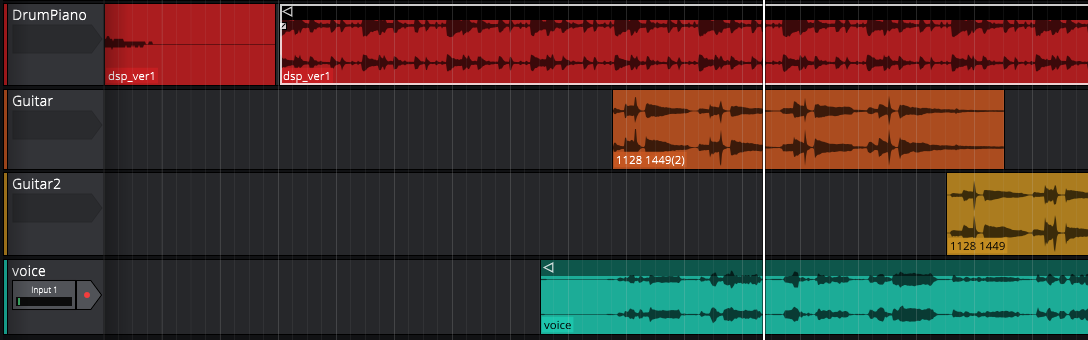
\includegraphics[width=6 in]{../pic/MySongProj.png}
	\caption{My Song Project}
	\label{fig:MySongProj}
\end{figure}

\newpage

\subsection{Lyrics}

This song is actually about what I am thinking while going back home.
Here is my lyrics:

\begin{quotation}
I miss the sun

I miss the moon

I miss the cloud

I miss the rain

I miss you mom

I miss you dad

I miss my toys

I miss my bed

You see the plane

You see the train

You hear my words

that I'm going away

Now I am back

Now I am back

I'm on my way

singing this song

Soon I will go

Soon I will go

All I can do

is singing this song
\end{quotation}

\subsection{Inspiration}

I was inspired by how the time flies, and the fact that my time to meet parents may be shorter and shorter. As I wrote at the end of the lyrics, I sing this song to enjoy the joy of going home, and also sing this song to relieve the sadness of leaving home

\section{Receiver}
\subsection{Circular Convolution}

Since the circular convolution is actually a product sum of tow sequences, we can represent the result using matrix multiplication. We can find the calculation rules that should be used in the following two cases by finding the patterns. 

For example, if we have 
\begin{gather*}
	h = [1, 2, 3, 4, 5] \\ 
	x = [1, 3, 5] \\ 
	\mathrm{len}(h) > \mathrm{len}(x)
\end{gather*}

The circular convolution can be represented as below, the $(a_1, a_2, a_3) \cdot (b_1, b_2, b_3)$ represents $a_1\times b_1 + a_2 \times b_2 + a_3 \times b_3$
\begin{align*}
[& \\ 
&(4, 5, 1) \cdot (5, 3, 1) ,\\ 
&(5, 1, 2) \cdot (5, 3, 1), \\ 
&(1, 2, 3) \cdot (5, 3, 1), \\ 
&(2, 3, 4) \cdot (5, 3, 1), \\ 
&(3, 4, 5) \cdot (5, 3, 1) \\ 
]&
\end{align*}
we can rearrange it as below
\begin{align*}
[& \\ 
&(1, 5, 4) \cdot (1, 3, 5) ,\\ 
&(2, 1, 5) \cdot (1, 3, 5), \\ 
&(3, 2, 1) \cdot (1, 3, 5), \\ 
&(4, 3, 2) \cdot (1, 3, 5), \\ 
&(5, 4, 3) \cdot (1, 3, 5) \\ 
]&
\end{align*}

So, the circular convolution can be represented as below
$$
H \cdot x^T = 
\begin{bmatrix}
	1 & 5 & 4 & 3 & 2 \\
	2 & 1 & 5 & 4 & 3 \\ 
	3 & 2 & 1 & 5 & 4 \\ 
	4 & 3 & 2 & 1 & 5 \\ 
	5 & 4 & 3 & 2 & 1
\end{bmatrix}
\cdot
\begin{bmatrix}
	1 \\ 
	3 \\ 
	5 \\ 
	0 \\ 
	0 
\end{bmatrix}
= 
\begin{bmatrix}
	36 & 30 & 14 & 23 & 32
\end{bmatrix}
$$

It is easy to get the $H$ matrix, we only need to write the first column in the order of $h[0] \to h[M - 1] $, the columns after the first column is just a shift of the first column.

So, also, if we have
\begin{gather*}
	h = [1, 2, 3] \\ 
	x = [1, 3, 5, 7] \\ 
	\mathrm{len}(h) < \mathrm{len}(x)
\end{gather*}
then we try to follow the same rule and fill the blank with $0$
$$
H \cdot x^T =
\begin{bmatrix}
	1 & 0 & 3 & 2 \\ 
	2 & 1 & 0 & 3 \\ 
	3 & 2 & 1 & 0 \\ 
	0 & 3 & 2 & 1
\end{bmatrix}
\cdot 
\begin{bmatrix}
	1 \\ 
	3 \\ 
	5 \\ 
	7
\end{bmatrix}
=
\begin{bmatrix}
	30 & 26 & 14 & 26
\end{bmatrix}
$$
the result is correct as well. So we can say this method of calculating circular convolution is correct.

\subsection{Calculation the Original Signal}
Known from the last subsection, signal after the wireless channels can be represented as the circular convolution of $x$ and $h$. Moreover, the circular convolution can be calculated as below
$$
h \, \otimes \, x = H \cdot x^T
$$
If $H \cdot x^T$ is known, to calculate the $x$ is to calculate the $H^{-1}$.

So, just follow the rule shown in the last subsection, we can calculate the original $x$ from $h \, \otimes \, x$.

For example, we have
\begin{gather*}
	h = [1, 2, 3] \\ 
	x = [1, 3, 5, 7, 9] \\ 
	y = H \cdot x^T = [30 , 26 , 14 , 26]
\end{gather*}

So we should first calculate the $H^{-1}$ as below
$$
H^{-1} = 
\left[ 
\begin{matrix}
	1 & 0 & 3 & 2 \\ 
	2 & 1 & 0 & 3 \\ 
	3 & 2 & 1 & 0 \\ 
	0 & 3 & 2 & 1
\end{matrix}
 \right]^{-1}
$$
then, the $x$ is as below
$$
x = H^{-1} \cdot y
$$

The verifying code is in the appendix part.

\bibliographystyle{ieeetr}
\bibliography{../bib/database}



\begin{appendices}
\section{Code Listing}
\begin{python}
import numpy as np

def createMat(x):
    N = len(x)
    mat = np.zeros([N, N])
    for i in range(N):
        tmp = np.roll(x, i)
        mat[i] = tmp
    return np.transpose(mat)

def regulateVector(x, h):
    lx = len(x)
    lh = len(h)
    if (lx > lh):
        h = np.concatenate((h, np.zeros(lx -lh)))
    elif (lx < lh):
        x = np.concatenate((x, np.zeros(lh - lx)))
    return x, h

# x, h generation
N = 500
M = 400
x = np.random.randn(N)
h = np.random.randn(M)
x, h = regulateVector(x, h)

# create the H matrix and calculate the reverse of it
H = createMat(h)
H_r = np.linalg.inv(H)

# calculate the circular convolution and do the reverse work
y = np.matmul(H, x)
ix = np.matmul(H_r, y)

# test the algorithm
print(np.mean(x - ix))
# the output is -1.3596658521297655e-15
\end{python}
\end{appendices}

\end{document}